%\documentclass{article}
%\usepackage{amssymb}
%\usepackage{wasysym}
%\usepackage{graphicx}
%\usepackage{bm}
%\usepackage{psfig}
%\newcommand{\bc}{\begin{center}}
%\newcommand{\ec}{\end{center}}
%\newcommand{\be}{\begin{equation}}
%\newcommand{\ee}{\end{equation}}
%\newcommand{\bea}[1]{\begin{eqnarray}\label{#1}}
%\newcommand{\eea}{\end{eqnarray}}
%\newcommand{\bua}{\begin{eqnarray*}}
%\newcommand{\eua}{\end{eqnarray*}}
%\newcommand{\infint}{\int_{-\infty}^{\infty}}
%\newcommand{\dd}[2]{{{d#1}\over{d#2}}}
%\newcommand{\ddt}[1]{\dd{#1}{t}}
%\newcommand{\dddt}[1]{\dd{^2#1}{t^2}}
%\newcommand{\aver}[1]{\langle{#1}\rangle}
%\def\cl#1{{\cal #1}}               % for caligrafic letters
%\def\labs{\mid\!}
%\def\rabs{\!\mid}
%\begin{document}
%\setcounter{section}{8}
\chapter{Imaging}

\section{The inverse problem}

A problem that occurs throughout astronomy is how best to interpret noisy data so that the resulting deduced quantities are real and not artifacts of the noise. This problem is termed the inverse problem. 

Spurious features may be removed from the image if the effects of the imperfections are known. But since there is uncertainty in both the data and the measurements of the imperfections, there can remain the possibility that features in the final image are artifacts of the noise, or are are incompletely removed.

Even a faultlessly constructed telescope will spread the image of a true point source into the Airy diffraction pattern. If the effect of the instrument and other sources of blurring on a point source or its equivalent is know, {\it i.e.} the PSF as defined below, then an attempt may be made to remove its effect from the data. If we consider a single linear optical device, then we can relate the output field $\psi_2$ at $z_2$ to the input $\psi_1$ at $z_1$ using a {\it Greens' function} denoted $P_{21}({\bf x}_2,{\bf x}_1))$: 
\[
\psi_2({\bf x}_2)=\int P_{21}({\bf x}_2,{\bf x}_1)d^2x_1\psi_1
\]
If $\psi_1$ were a $\delta$-function, then the output would be simply given by the function $P_{21}$, up to a normalization. Thus, $P_{21}$ is known as the {\it Point Spread Function} or PSF. The process of removing instrumental effects form data can be necessary for any type of measurement, but is perhaps best studied in relation to imaging, when the process is generally known as de-convolution.

\subsection{De-convolution}

The true image {\it convolves} with the PSF to give the observed image. Inversion of this effect is thus deconvolution. This is most easily illustrated by considering a one-dimensional case. 

A one dimensional image, such as a spectrum, may be completely represented by a plot of its intensity against the distance along the image. The PSF may be similarly plotted and may be found, in the case of a spectrum by observing the effect of the spectroscope on a monochromatic source. 

If we regard the true spectrum as a collection adjoining monochromatic intensities, then the effect of the spectroscope will be to broaden each monochromatic intensity into the PSF. At at given point in the observed spectrum, some of the original energy will have been displaced out to nearby wavelengths, while energy will have been added from the spreading out of nearby wavelengths. This process can be written mathematically as the convolution
\be
O(\lambda_1)=\int_0^{\infty} T(\lambda_2)I(\lambda_1-\lambda_2)d\lambda_2=T\otimes I
\label{eq:convolution}
\ee
Where $O(\lambda_1)$ is the intensity in the observed spectrum at $\lambda_1$, $T(\lambda_2)$ is the intensity of the true spectrum at $\lambda_2$, and $I(\lambda_1-\lambda_2)$ is the response of the instrument at a distance $(\lambda_1-\lambda_2)$ from the center.

To invert equation~\ref{eq:convolution} we take its Fourier transform $\cl{F}(O)$ such that
\be
\cl{F}(O)=\cl{F}(T\otimes I)=\cl{F}(T)\times\cl{F}(I).
\label{eq:fourier-convolution}
\ee
The true spectrum (image or other observable) may be found by taking by inverting equation~\ref{eq:fourier-convolution} and then taking the inverse Fourier transform
\[
T=\cl{F}^{-1}\left[{\cl{F}(O)\over\cl{F}(I)}\right].
\]

In practice, there are two difficulties in following this process. First data is sampled at discrete intervals and so is not the continuous function required to complete the Fourier transform, and also it is not available over the complete range from $-\infty$ to $+\infty$. Second the presence of noise will produce ambiguities in the calculated values of $T$.

The first problem can be overcome by using the discrete versions of the the Fourier transforms as shown in lecture notes 4 on Fourier transforms. Remember that a that has 
a maximum frequency of $f$ is completely determined by sampling at $2f$ according to the sampling theorem. Thus, the use of the discrete form of the Fourier transform involves no loss of information providing that the sampling frequency (${1/\Delta}$) is twice the highest frequency in the source function. If the source function contains frequencies higher than the Nyquist frequency (${1/2\Delta}$), then these will not be determined by the measurements and the finer detail in the source function will be lost. More seriously, the higher frequency components may beat with the measuring frequency to produce spurious components of frequencies lower than the Nyquist frequency. This phenomenon is known as aliasing. 

Some reduction in the noise in the data may be achieved by operating on its Fourier transform. For example, random noise may be reduced by using the optimal (or Wiener) filter defined by 
\[
W={[\cl{F}(O)]^2\over[\cl{F}(O)]^2+[\cl{F}(N)]^2}
\]
where $\cl{F}(O)$ is the Fourier transform of the observations, without the effect of noise, and $\cl{F}(N)$ is the Fourier transform of the random noise. The noise and the noise free signal are separated by assuming the high frequency tail of the power spectrum to be just noise, and then extrapolating linearly back to the lower frequencies. Equation~\ref{eq:fourier-convolution} becomes
\[
T=\cl{F}^{-1}\left[{\cl{F}(O)W\over\cl{F}(I)}\right].
\]
\subsection{MOMFBD}

\section{Photography}
Photography is hardly used at all in professional astronomy --- the last photograph on the AAT was taken in 1999, for example. CCDs now dominate imaging from the ultraviolet to the near infrared. However, photography is perhaps not totally dead, Kitchin's {\it Astrophysical Techniques} contains good descriptions of photographic process.

\section{Scanning}

Scanning is a quite obvious way of building up a two dimensional image which may be built up by using a point source detector, if the detector is scanned over the image or vice versa. Scanning patterns are normally raster or spiral. Other patterns may also be encountered. Many Earth observation satellites use {\it push-broom} scanning, in which a linear array of detectors is aligned at right angles to the spacecraft's ground track. The image is built up at the spacecraft's motion move the array to look at successive slices of the swathe of ground over which the satellite is passing.

A more sophisticated technique is to modulate the output of the detector by interposing a mask of some type in the light beam, as previously discussed in the lecture 8 notes on high energy astrophysics where we described modulation collimators and the coded array mask used in x-ray imaging. An improved method is known as Hadamard mask imaging. Its principles can be illustrated by considering one-dimensional images. The mask is placed in the image plane of the telescope, and a lens directs all the light from to a single detector. Thus the output from the system consists of a simple measurement of the intensity passed by the mask. If a different mask is substituted for the first, then a new and in general different reading will be obtained. If the image is to be resolved into
$N$ elements, then $N$ such different masks must be used, and $N$ intensity readings determined. If ${\bf D}$ is the vector formed from the detector output, ${\bf I}$ is the vector of intensities of the elements of the image, and ${\bf M}$ the $N\times N$ matrix whose columns each represent one of the masks, then ignoring noise we have
\[
{\bf D}={\bf IM}
\]
and so 
\[
{\bf I}={\bf DM}^{-1}.
\]
Thus the original image is obtained by inverting the matrix representing the mask. The improvement over this method over a simple scan lies in its multiplex advantage. The masks usually comprise segments that either transmit or obscure the radiation completely 
\[ 
m_{ij}=0 \quad {\rm or} \quad 1.
\]
and, on average, about half the total image is obscured by a mask. Thus $N/2$ image segments contribute to the intensity falling on the detector at any one time. Hence, if 
a given signal to noise ratio is reached in a time $T$, when the detector observes a single image element, then the total time required to detect the who image with simple scans is $N\times T$ and is only $\sqrt{2N}T$ for the Hadamard masking system. Thus, the multiplex advantage is approximately $\sqrt{N/2}$ improvement in the exposure length. 

One method of finding suitable matrices to reduce construction costs and noise is based on a group of matrices known as the Hadamard matrices (hence the name of the method). These are matrices whose elements are $\pm 1$ and which have the property
\[
{\bf H}{\bf H}^{\rm T}=N{\bf I}
\]
where ${\bf H}$ is the Hadamard matrix and ${\bf I}$ is the identity matrix. 

\section{Interferometry}

The simplest example of interference is given by Young's slits. Suppose two long,
narrow, parallel slits are illuminated coherently by monochromatic light from a distant
source that lies on the perpendicular axis between the two slits (the optic axis) so that the incident wavefront reaches the slits simultaneously. The waves from the slits fall onto a screen in the distant, Frauenhofer region, and there they interfere. The Frauenhofer 
interference pattern observed at a point $\cl{P}$, at position $r,\theta$, is proportional to the spatial Fourier transform of the transmission function. If the slits are 
narrow, we can regard the transmission function as two $\delta$-functions, separated
by the slit spacing $a$, and its Fourier transform will be
\[
\psi_{\cl{P}}\propto e^{-ika\theta/2}+e^{ika\theta/2}\propto\cos\left({ka\theta\over 2}\right).
\]
The energy flux at point $\cl{P}$ is the square of this
\[
F_{\cl{P}}\propto\labs\psi\rabs^2c\propto\cos^2({ka\theta/2}).
\]
The alternating bright and dark illumination in this flux distribution are known as {\it interference fringes}. 

Let us now consider an extended source: Keep the incoming waves perfectly 
coherent and perfectly planar, but change their incoming direction so that it makes a small angle $\alpha$ to the optic axis. Then the distribution of the energy flux in the
Frauenhofer diffraction pattern on the screen will be modified to 
\bua
F_{\cl{P}}&\propto&\labs e^{-ika(\theta-\alpha)/2}+e^{ika(\theta-\alpha)/2}\rabs^2
      \propto\cos^2\left[{ka(\theta-\alpha)\over 2}\right] \\
             &\propto& \{1+\cos[ka(\theta-\alpha)]\}.
\eua
Notice that as the direction $\alpha$ of the incoming wave changes, the locations $\theta$ of the bright and dark fringes change. Thus the positions of the fringes carry information about the direction to the source. 

An extended source is one whose radiation comes from a finite range of angles $\alpha$, let us assume $\alpha\ll 1$. Assume further that the source is monochromatic (this can be achieved by filters if necessary), but we will allow the source to have a 
randomly fluctuating phase $\delta\phi(t)$ in keeping with all realistic monochromatic sources, and shall require that the time-scale on which the phase wanders (the waves coherence time) be very long compared to the waves' period $2\pi/\omega_0$. It is also assumed that, as for most realistic sources, the fluctuating phases in the waves from different directions are completely uncorrelated. The field is then written in the 
form
\[
\psi=e^{ik(kz-\omega_0t)}\int\psi(\alpha,t)e^{ik\alpha x}d\alpha
\]
where $\psi(\alpha,t)=Ae^{-i\delta\phi}$ is the slowly wandering complex amplitude of the waves from direction $\alpha$. When considering the total flux arriving at a given point $(x,z)$ from two different directions $\alpha_1$ and $\alpha_2$ and average it over times long compared to the waves' coherence time, all interference between the two contributions and they superpose incoherently which means that their intensities averaged over time add linearly.

Thus the angularly incoherent light from our extended source is sent through two Young's slits and produces fringes on a screen. Assuming that the coherence time for the
light from each source point is very long compared to the difference in light travel time
 to the screen via the two different slits. Then the light from each source point in the 
extended source forms sharp interference fringes. However, because contributions from the different directions add incoherently, the flux distribution on the screen is a linear sum of the fluxes from all the source points
\[
F_{\cl{P}}\propto\int d\alpha I(\alpha)\{1+\cos[ka(\theta-\alpha)]\}
\]
where $I(\alpha)d\alpha\propto\overline{\labs\psi(\alpha,t)\rabs^2}d\alpha$ is the flux incident on the plane of the slits form the infinitesimal range $d\alpha$ of directions. Presume that the range of angles present in the wave, $\Delta\alpha$, is large compared to their bandwidth $\Delta\alpha\gg{\Delta\omega/\omega_0}$ so whereas the finite but tiny bandwidth produced negligible smearing out of the interference fringes, the finite but small range of directions may produce significant smearing and the minima of $F_{\cl{P}}$ might not be very sharp. The fringes non-sharpness and their locations can be quantified by writing the slit produced flux distribution as
\[
F_{\cl{P}}=F_S[1+\cl{R}\{\gamma_\perp(ka)e^{-ika\theta)}\}]
\]
with
\[
F_S\equiv\int d\alpha I(\alpha)
\]
is the total flux arriving at the slits from the source, and 
\be
\gamma_\perp(ka)\equiv{\int d\alpha I(\alpha)e^{ika\alpha}\over F_S}
\label{eq:spatial-coherence}
\ee
is known as the radiation's {\it degree of spatial coherence}. The phase of $\gamma_\perp$ determines the angular locations of the fringes; its modulus determines their depth. 

Equation~\ref{eq:spatial-coherence} says that the degree of spatial coherence from an extended, angularly incoherent source is the Fourier transform of the source's angular intensity pattern. Correspondingly, if one knows the degree of spatial coherence as a function of the distance $ka$, from it one can reconstruct the source's angular intensity pattern by Fourier inversion:
\be
I(\alpha)=F_S\int{d(ka)\over 2\pi}\gamma_\perp(ka)e^{-ika\alpha}.
\label{eq:fourier-coherence}
\ee

For a given choice of $ka$, {\it ie} a given distance between the slits, $\gamma_\perp$ is a complex number that one can read off the interference fringes as follows: Its modulus is 
\[
\labs\gamma_\perp\rabs\equiv V={F_{\rm max}-F_{\rm min}\over F_{\rm max}+F_{\rm min}}
\]
where $F_{\rm max}$ and $F_{\rm min}$ are the maximum and minimum values of the flux $F_{\cl P}$ on the screen; and its phase ${\rm arg}(\gamma_\perp)$ is $ka$ times the displacement $\Delta\theta$ of the centers of the bright fringes from the optic axis. The modulus is called the fringe {\it visibility} because of it measuring the fractional contrast in the fringes. 

\subsection{Michelson Stellar Interferometer}

Michelson's stellar interferometer implements Young's slits for measuring spatial coherence which Michelson used for measuring the angular diameters of Jupiter's 
moons and some bright stars in 1920 and a bit earlier. The light is sampled at two 
small mirrors separated by a variable distance $a$ and then reflected onto a telescope 
to form interference fringes. It is found that as the separation $a$ between the mirrors 
is increased, the fringe visibility decreases. If we model a star as circular disk of 
uniform brightness, then the degree of spatial coherence of the light from it is given
as 
\[
\gamma_\perp=2{\rm jinc}(ka\alpha_r)
\]
where $\alpha_r$ is the angular resolution of the star and 
${\rm jinc}(\xi)={J_1(\xi)/\xi}$. Michelson found that for the star Betelgeuse observed
at a wavelength $\lambda=570$~nm, the fringes disappeared when $a\sim 3$~m. 
Associating this with the first zero of the function ${\rm jin}c(x)$, Michelson inferred that
the angular radius of Betelgeuse is $\sim 0.02$~arcsec, which at Betelgeuse's distance
200~pc corresponds to a physical radius $\sim 300$~$R_S$.

In practice this type of interferometer uses the outputs fro many telescopes. However, this is only to reduce the time taken for observations, and it is actually the outputs from pairs of telescopes that are combined to produce the interference effects. Let us compare the resolution achieved with a telescope of diameter $D$ with an interferometer: For an telescope of diameter $D$ two source are separable if their angular separation is larger than the Rayleigh criterion of
\[ 
\alpha'={1.22\lambda\over D}.
\]
\noindent
On the other hand the fringe pattern given by two sources separated by 
\[
\alpha''={\lambda\over 2d},
\]
\noindent
where $d$ is the separation between the two Young's apertures, will disappear. The fringe pattern will reappear again for an angle $2\alpha''$ and disappear again for $3\alpha''$. Thus the resolution of two apertures is given by the separation of the sources for which the two fringe systems are mutually displaced by half a fringe width. This is given by the angle $\alpha''$ and the comparison between the telescope and interferometer gives
\[
{\alpha''\over\alpha'}={D\over 2.44d}
\]
\noindent
The resolution of the interferometer is almost 2.5 times that of a telescope with the same diameter for point sources! 

\begin{figure}[h]
  \centering
%	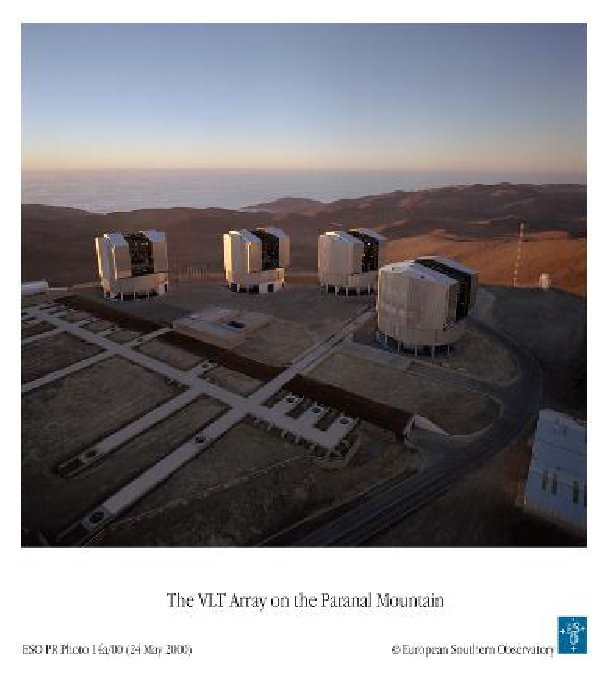
\psfig{file=vlt-image-smallsize.eps,width=0.75\textwidth}
	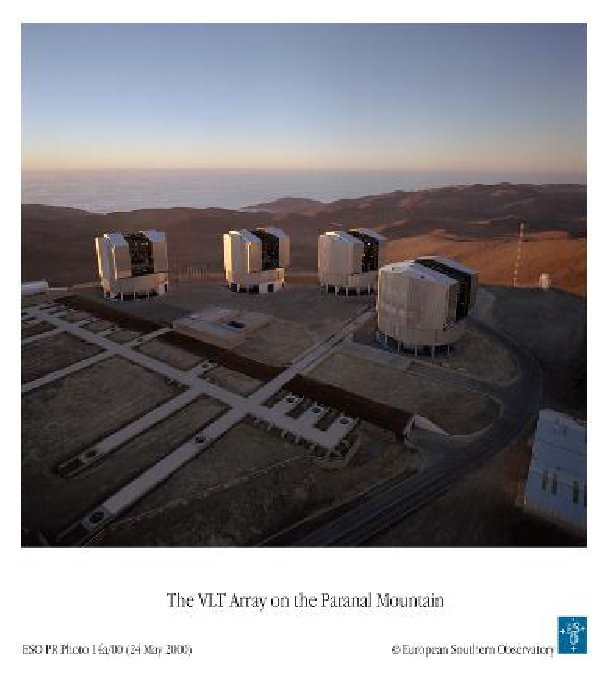
\includegraphics[width=0.75\textwidth]{vlt-image-smallsize.eps}
  \caption{The VLT Array on the Paralal Mountain which can be used as a stellar interferometer.}
  \label{fig:vlt-array}
\end{figure}

In order to produce fringes with maximum clarity, the path difference must be close to zero. This is because radiation is never completely monochromatic; any signal will have a certain bandwidth $\Delta\lambda$. For zero path difference at the apertures, all wavelenghts will be in phase, and they will interfere constructively. If the path difference is not zero, some wavelengths will be in phase but others will be out of phase since the path difference will equal different numbers of cycles or fractions of cycles at different wavelengths. There will therefore be a mix of constructive and destructive interference, and the observed fringes will have reduced contrast. The path difference for which the contrast in the fringes reduces to zero ({\it i.e} no fringes) is called the coherence length, $l$, given by
\[
l={c\over\Delta\nu}={\lambda^2\over\Delta\lambda}
\]
\noindent
For $\lambda=500$~nm and $\Delta\lambda=1$~nm, we have a coherence length of
0.25~mm, for white light $\lambda=300$~nm this reduces to less than a $\mu m$, but in the radio region it can be large; at $\nu=1.5$~GHz and $\Delta\nu=10$~MHz it is fully 30~m. The path difference to the apertures, or their equivalent, must be kept to a small fraction of the coherence length. Michelson acheived this by the use of adjustable glass wedges in his interferometer where the path difference was small. However, modern telescopes can be over 100~m apart for optical telescopes and up to thousands of kilometers for very-long-baseline radio interferometry, and a complex system of delay lines must be built in order to achieve coherence, or alternately afterwards during data processing in the case of radio observations where also the phase can be recorded.

Very stringent requirements on the stability and accuracy are required in order for this technique to work. The path difference of the slits must not be greater than a small fraction of the coherence length. %furthermore that path difference must remain %constant to considerably better than the wavelenght of the radiation that is being used %as the slits are separated. 
Vibrations and scintillation are additional limiting factors.

A proposal for the future is to use {\it nulling interferometry} based in space. This would use destructive interference to supress the bright central object in order to look for the much dimmer companions such as Earth-like planets. To achieve this around stars 10~pc or more away one would need baselines of order 50~m and observations taking a few hours with a four element array of telescopes.

\subsection{Michelson radio interferometer}

There is no difference in principle between a radio and an optical interferometer when they are used to measure the separation of double source, or the diameters of uniform objects. However, the output from a radio telscope contains both the amplitude and the phase of the signal, so that complete imaging of the source is possible. This is achieved by using equation~\ref{eq:fourier-coherence} to perform the Fourier inversion of the lateral degree of coherence $\gamma_\perp({\bf a})$, which must be measured for a 
variety of values of the relative separatioin vector ${\bf a}$ of the telescopes perpendicular to the direction of the source. As the earth rotates, this vector will trace out half an ellipse in the two-dimensional ${\bf a}$ plane every twelve hours. Since the source intensity is real equation~\ref{eq:fourier-coherence} implies that $\gamma_\perp(-{\bf a})=\gamma_\perp^*({\bf a})$. By changing the spacing between the telescopes the degree of coherence can be well sampled. In practice a modern interferometer has many more than two telscopes. The Very Large Array (VLA) in New Mexico has 27 individual telescopes arranged in a `Y' pattern and operating simultaneously. The degree of coherence can thus be measured simultaneously over 
${27\times 26/2}=351$ different relative separations. The maximum baseline of the VLA is 36~km.

\paragraph{Closure phase.}

\subsection{Speckle interferometry}

Speckle interferometry works by obtaining images of the object sufficiently rapidly to freeze the blurring of the image that arises from atmospheric scintillations. The total image then consists of a large number of small dots or speckles, each of which is a diffraction-limited image for some objective diameter up to and including the diameter of the actual objective.

Consider the effect of seeing upon the wavefront of the object. Assume that the wavefront is initially planar and coherent, then the main effect of scintillation is to introduce differential phase delays across it. A typical cell size is 0.1~m and the scintillation frequency is in the range 1 -- 100~Hz. Thus some 100 atmospheric cells will affect an average image from a 1~m telescope at any given instant. These will be rapidly changing. An exposure of a few milliseconds will freeze the image motion, and the observed image is then just the resultant of the contributions from the atmospheric cells across the telescope objective at the moment. The large number of cells renders it highly probable that some of the phase delays will be similar and so some of the contributions to the image will be in phase with each other. These particular contributions will have been distributed over the objective in a random manner. Considering two such contributions, we have a simple interferometer, and the tow beams of radiation will combine in the image plane to produce results identical with those of an interferometer whose baseline is equal to the separations of the contribution on the objective. The smallest speckles in the total image therefore have the diffraction limited resolution of the whole objective. 

%\end{document}
